
	\section{ACM/ICPC World Finals 2005}
		\subsection{ACM/ICPC World Finals 2005 B Simplified GSM Network}
			\subsubsection{题目大意}
				如图 \ref{2005b},有若干基站与城市。城市之间有笔直的道路。问城市 $u$ 沿道路 到 城市 $v$,手机最少要切换几次基站?手机总寻找最近的基站。
				\begin{figure}[htb]
					\centering
					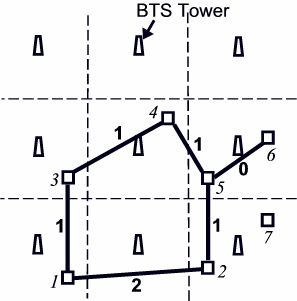
\includegraphics[width=0.3 \textwidth]{2005b.png}
					\caption{基站为梯形,城市为方形} \label{2005b}
				\end{figure}

				基站数 $N \le 50$, 城市数  $M \le 50$,道路数 $K \le 250$, 询问数  $Q \le 10$。道路不会与基站服务范围重合成一条线段。
			\subsubsection{算法讨论}
				根据计算几何,可在
%				先
				求出基站的 Voronoi 图后,与道路求交,将相交次数作为边权,带回原问题,即可用最短路算法求知答案。
				
				但是,求  Voronoi 图 的算法十分复杂,而我们可以避开它 ,不直接求出 Voronoi 图,将  Voronoi 图与道路相交的次数求出。
				
				 Voronoi 图 中所有的线段都是两点的中垂线,故我们先枚举两个基站,求出其中垂线,与道路求交,可能会得到一个交点。如果确实得到了此交点,那么还需判断其是否在 Voronoi 图 上(因为可能在 Voronoi 图 中 这条线段的延长线上),方法是求出这点与其他基站的最短距离,判断这个距离是否为该点到这两个选择的基站的距离。如果不是,那么这个点仍需排除;否则,这个点就是 Voronoi 图与道路的交,权值自增一。
				
				求出边权后,使用最短路算法即可。
			\subsubsection{时空复杂度}
				时间复杂度 $\mathcal{O}\left(N^2K + M^3 + K\right)$。
					
				空间复杂度 $\mathcal{O}\left(N + M^2)\right)$。
		\newpage
		\subsection{ACM/ICPC World Finals 2005 C The Traveling Judges Problem}
			\subsubsection{题目大意}
				给定无向图 $G=(V, E)$,边权 $W: E \mapsto \mathbb{R}^{+}$ ,有 $N_0$ 个人,分别位于 $s_1, s_2, \ldots, s_{N_0}\in V$,均前往同一目的地 $t \in V$。他们可以打无数个的,每个的可容纳无数人,且仅以路程(边权之和)正比例地计费
%				,无起步价,燃油,保险,空程,多人等的收费
				。问他们需要多少钱就可以共同到达目的地?并输出方案。
				
				$N = |V| \le 20, N_0 \le 10
%				, M = |E| \le
				$。
			\subsubsection{算法讨论}
				不妨将他们经过的点标记出来,将其他的点剔除,求最小生成树。可以说明最小生成树的权值就是答案。因为他们都经过了这些点,而进一步缩小答案就会导致图不连通,与假设矛盾;而就以 $t$ 为根,只要这些人都往父亲结点方形走,并在每一条边都与要经过这条边的人和打一辆的即可,答案是足够的。
				
				枚举 $2^N$ 种情况求最小生成树判断即可。记录下最优解的最小生成树就可以输出方案了。
			\subsubsection{时空复杂度}
				时间复杂度 $\mathcal{O}\left(N^2\log N + 2^N \cdot N^2 \right)$。
					
				空间复杂度 $\mathcal{O}\left(N^2\right)$。
		\newpage
		\subsection{ACM/ICPC World Finals 2005 D cNteSahruPfefrlefe}
			\subsubsection{题目大意}
				设有一碟扑克牌  $a_1, a_2, \ldots, a_N$, $N$ 是扑克牌的总张数。一个完美的洗牌是指将这个序列变成
				\begin{align}
					a_{27},  a_1, a_{28}, a_2, \ldots, a_N, a_{N-1}  \label{2005d}
				\end{align}
				一次不完美的洗牌 
				是指形成 \eqref{2005d} 中相邻两项被交换后的结果。
				
				一开始的牌是整齐的 , $a_i = i$。某人连续洗了\emph{不超过} $K$ 次牌,每次都只是完美的或不完美的。给出洗完牌
%				都
				的结果,问每一次洗牌中那些是不完美的,并指出不完美的洗牌中,哪两张牌被交换了。
				
				$N = 52, K = 10$。
			\subsubsection{算法讨论}
				如果直接对次问题建立数学模型,可以发现就是若干置换(完美洗牌),插入一些两个元素的置换(不完美洗牌的交换),使得形成目标置换。经过化简后就可得知,问题就是选择若干只有两个元素的置换相乘,使得形成一个目标置换。简单的说,给定一排打乱的元素,交换不超过 $K$ 次,每次换两个元素,请将其交换成	
%				一个
				一排有序的元素。
				
				由于 $K = 10$,那么可以先枚举此人真正交换元素的次数 $K_0$,再爆搜(迭代加深),每次有 $\binom{52}{2}$ 种交换方法,故总情况数 $\binom{52}{2}^{K_0}$。存在一个减枝,如果目前仅剩余 $x$ 次交换,但有多于 $2x$ 的元素没有回到正确的位置,这时肯定无解,可直接返回。
			\subsubsection{时空复杂度}
				时间复杂度 $\mathcal{O}\left(\binom{N}{2}^K \right)$。
					
				空间复杂度 $\mathcal{O}\left(N\right)$。
		\newpage
		\subsection{ACM/ICPC World Finals 2005 E Lots of Sunlight}
			\subsubsection{题目大意}
				如图 \ref{2005e},给出若干栋楼房的位置,且均位于同一个东西方向的竖直平面。给定当天日出日落的时间,太阳以某一常角速度运动,阳光视为平行光。问其中一些房间那些时刻有阳光照射(某一侧窗完全被照到)?
				\begin{figure}[htb]
					\centering
					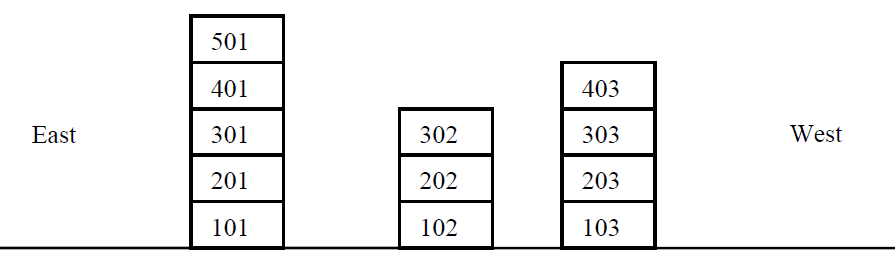
\includegraphics[width=0.7 \textwidth]{2005e.png}
					\caption{} \label{2005e}
				\end{figure}
				
				建筑 $N < 100$
%				,询问数 $M \le $
				。
			\subsubsection{算法讨论}
				求出要询问的房间所在的建筑编号。枚举比这栋楼高的其他建筑,确定该房间的阳光被这栋枚举的楼挡住的临界时间。方法是求出房间左(右)下角与枚举的楼的右(左)上角连线的倾角,除上太阳角速度极为时间,具体取哪个方向视枚举的建筑与房间的左右关系确定。
				
				临界时间决定了有阳光照射的上(下)限(也根据建筑与房间的左右关系确定),这样就能确定答案区间,转换为时分秒格式输出。
			\subsubsection{时空复杂度}
				单次询问时间复杂度 $\mathcal{O}\left(N \right)$。
					
				空间复杂度 $\mathcal{O}\left(N\right)$。

\newpage
		\subsection{ACM/ICPC World Finals 2005 F Crossing Streets}
			\subsubsection{题目大意}
				例如图 \ref{2005f},给定地图信息,马路均为平行于坐标轴的线段。\emph{不能穿过十字路口},问从家到学校至少须穿过多少次马路?
				\begin{figure}[htb]
					\centering
					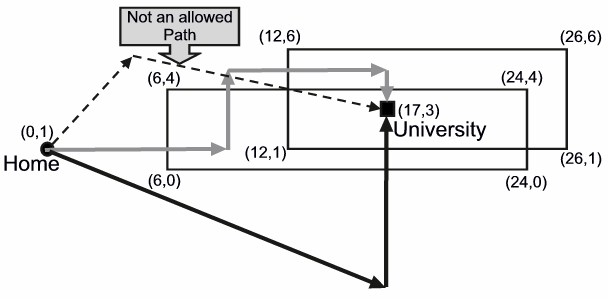
\includegraphics[width=0.7 \textwidth]{2005f.png}
					\caption{} \label{2005f}
				\end{figure}
				
				马路数 $n \le 500$。
			
			\subsubsection{算法讨论}
				将马路延长后,可得到一个 $N \times M$ 的网格,且  $\mathcal{O}(n) = \mathcal{O}(N) = \mathcal{O}(M) $。实现的过程中,不必实际地将其直接延长,而可使用 时间复杂度 $\mathcal{O}(n \log n)$ 的离散化实现。
				
				这样转化成网格后,问题等价于,从一个格子仅通过相邻的格子走到另一个格子,部分相邻格子间无代价,部分相邻格子间代价为 $1$,问最小代价。这可以用传统的 BFS 算法解决,但与传统做法稍有不同的是,必须先访问代价为 0 的点,再访问代价为 $1$ 的点,这样才能保证队列
%				中的点
				代价单调。BFS 后终点格子的权值就是答案。
			\subsubsection{时空复杂度}
				时间复杂度 $\mathcal{O}\left(n^2 \right)$。
					
				空间复杂度 $\mathcal{O}\left(n\right)$。

\newpage
		\subsection{ACM/ICPC World Finals 2005 G Tiling the Plane}
			\subsubsection{题目大意}
				问一个简单\emph{正交}多边形在不旋转不翻转的情况下,是否能密铺平面。
				
				一个多边形能密铺平面当且仅当
				\begin{enumerate}
					\item 边界上存在有序的四点 $A,B,C,D$,使得有向的一段边界 $AB$ 与 有向边界 $DC$ 在平移后重合;或者
					\item 边界上存在有序的六点 $A,B,C,D,E,F$,使得有向的一段边界 $AB$ 与 有向边界 $ED$ 在平移后重合,且有向边界 $BC$  与有向边界 $FE$  平移后重合,还要有向边界 $CD$  与有向边界 $AF$  平移后重合。
				\end{enumerate}
				多边形顶点数 $n \le 50$。边界保证与坐标轴平行。
			\subsubsection{算法讨论}
				为了简化问题,不妨先将方向相同的两段相邻的边合并成一段。此操作不影响答案。
				
				为了高效地使用好题目给出的定理,我们预处理 $F[a][b][l]$ 表示从多边形顶点 $a$ 开始顺数 $l$ 个顶点的有向路径与 $b$ 开始倒数 $l$ 个顶点的有向路径的逆是否在平移后重合。此操作可在 $\mathcal{O}\left(n^4 \right)$ 的时间内实现——枚举 $a, b, l$ 耗时 $\mathcal{O}\left(n^3 \right)$,再模拟 耗时  $\mathcal{O}\left(n \right)$。
				
				不妨以第二条规则来阐述我们最终的判定算法,第一条规则同理。首先,如果答案为是,则要求 有向边界 $AD$ 的长度等于 有向边界 $DA$ 的长度。又多边形的总边数已经确定,换言之,确定了 $A$ 就确定了 $D$。同理, 确定了 $B, C$ 就确定了 $E,F$。这样枚举只需 $\mathcal{O}\left(n^3 \right)$ 时间。对于枚举出来的点的判定,只需求出相邻点间的长度 $l$,使用刚才预处理的 $F[\cdot][\cdot][\cdot]$,看看它们是否都为真。如果是,则立即返回能密铺;否则找不到这样的六元组,返回不能密铺。
				
				这个判定
%				规则
				法则
				的证明涉及到 \emph{希尔伯特第十八问题} 。笔者暂时无法给出该命题的证明。
			\subsubsection{时空复杂度}
				时间复杂度 $\mathcal{O}\left(n^4 \right)$。
					
				空间复杂度 $\mathcal{O}\left(n\right)$。


\newpage
		\subsection{ACM/ICPC World Finals 2005 H The Great Wall Game}
			\subsubsection{题目大意}

%				网格
				如图 \ref{2005h},大小 $n \times n$ 的网格中有若干棋子。每个棋子一次可往四个方向移动一步,且一个格子中不能同时存在两个棋子。问将其摆成以一横行,一纵列,或者一个对角线需至少移动几步?
				
				\begin{figure}[htb]
					\centering
					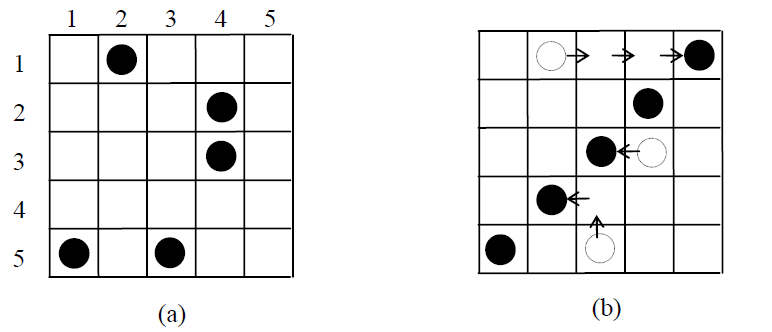
\includegraphics[width=0.7 \textwidth]{2005h.png}
					\caption{} \label{2005h}
				\end{figure}
				
				$n \le 15$。
			\subsubsection{算法讨论}
				分析可知 一个格子中是否可以同时存在两个棋子不影响答案,因为棋子之间没有分别,如果两个棋子互相穿越了对方,那么相当于在穿越对方的一瞬间角色互换,这样就不存在穿越事件了,而且这种情况下的答案可能会更小。不妨忽略此条件。
				
				问题即,给每个棋子分别指定一个终点,两两之间走最短路,代价为最短路之和。问什么样的指定方案最优?这样就是一个带权二分匹配的问题。枚举究竟是要在哪一行,哪一列,或者对角线设定终点,并抽象为左支的 $n$ 个点;再设 $n$ 个棋子为右枝的 $n$ 个点,左右支之间的点连边,代价为其间的最短路长度。答案即最小匹配的代价。
			\subsubsection{时空复杂度}
				时间复杂度 $\mathcal{O}\left(F(n) \right)$。 $F(n)$ 表示求解 $n$ 个点的带权完全二分图的最优匹配的时间,因具体使用的算法而异。
					
				空间复杂度 $\mathcal{O}\left(n^2\right)$。
				

\newpage
		\subsection{ACM/ICPC World Finals 2005 I Workshops}
			\subsubsection{题目大意}
				有 $N$ 个队伍,每个队伍有 $a_i$ 个人,需要开一个 $b_i$ 分钟的会议。同时有 $M$ 个房间,每个房间能容纳不超过 $A_i$ 个人,并只开放 $B_i$ 分钟,且最多被一个队伍使用。一个队伍最多使用一个房间。问最少有多少队伍不能参加会议;并在此基础上,最少有多少人不能参加会议。
				
				$N, M \le 1000$。
			
			\subsubsection{算法讨论}
				我们给出一个贪心算法 \ref{2005i}。
				\begin{algorithm}[H]
				\caption{}
				\label{2005i}
					\begin{algorithmic}[1]
						\For{按照 $B_i$ 从小到大的顺序枚举 $(A_i, B_i)$} 
								\State $S \gets \left\{a_j| a_j \le A_i, b_j  \le B_i, j \text{ 未曾被选择}\right\}$
								
								\If{
%									有这样的 $p$
								$S \ne \varnothing$
								}
									\State $p \gets S$ 中 $a_j$ 最大的 $j$。
									\State 将 $(a_p, b_p)$ 与  $(A_i, B_i)$ 配对,并标记 $p$ 被选择。
								\EndIf
%								答案为
						\EndFor
						\State 输出\emph{未被选择}的 $p$ 的数量及其 $a_p$ 之和。
					\end{algorithmic}
				\end{algorithm}	
				\begin{theorem}
					贪心算法 \ref{2005i} 能导出正确答案。
				\end{theorem}
				\begin{pf}
					我们假设某一个枚举的房间  $(A_i, B_i)$ 没有与最优的队伍 $(a_p, b_p)$ 配对,而与另一队伍  $(a_q, b_q)$  配对了。接下来分两种情况 
					\begin{enumerate}
						\item 如果    $(a_p, b_p)$   未与其他房间配对。注意到匹配的关系不会更改,那么使用调整法,直接将 $(A_i, B_i)$ 的对象更改为  $(a_p, b_p)$,不能参加会议的队伍数没变,不能参加会议的人不会变多,答案不会变差。
						\item 如果    $(a_p, b_p)$ 与 $(A_j, B_j)$  配对了。注意到 $(A_i, B_i)$  能匹配不优的   $(a_q, b_q)$,故
							$a_q \le a_p % \le A_i
						, b_q \le B_i$。又由于当时  $(a_p, b_p)$  未与其他房间匹配,可供   $(A_i, B_i)$ 选择,故一定有 $B_i \le B_j$。 $(A_j, B_j)$   配    $(a_p, b_p)$,故 $a_p \le A_j $ 合起来得到
							\begin{align}
								a_q \le a_p \le A_j \\
								 b_q \le B_i \le  B_j
							\end{align}
							故 $(a_q, b_q)$ 也能和 $(A_j, B_j)$ 配对。这样使用调整法直接交换这两对就可以得到新解,且答案不变化。
					\end{enumerate} 
					而如果   $(A_i, B_i)$ 没有与任何的队伍配对,那么直接把 最优的队伍 $(a_p, b_p)$  抢过来也能得到一个新解,答案不会变差。
					故总可以调整为  $(A_i, B_i)$ 与最优的队伍 $(a_p, b_p)$ 配对的较优解。
					
					重复上述过程,最终肯定可得到贪心解,而答案较初始解不会变差,又由初始解有任意性,综上,贪心算法 \ref{2005i} 能导出正确答案。\qed
				\end{pf}
					直接运行 贪心算法 \ref{2005i} 即可。
					\subsubsection{时空复杂度}
						时间复杂度 $\mathcal{O}\left(NM \right)$。
					
						空间复杂度 $\mathcal{O}\left(N + M\right)$。


\newpage
		\subsection{ACM/ICPC World Finals 2005 J Zones}
			\subsubsection{题目大意}

				如图 \ref{2005j},有
%				若干
				$N$ 个
				待建的基站,每个基站覆盖的范围是一个等圆。每个基站能服务的人数给定,同时有些基站之间有交集,也在输入中给出。选择开通哪 $M$ 个基站,能使得被服务的人数最多,并求出此人数。基站间的交集共有 $K$ 处。
				
				\begin{figure}[htb]
					\centering
					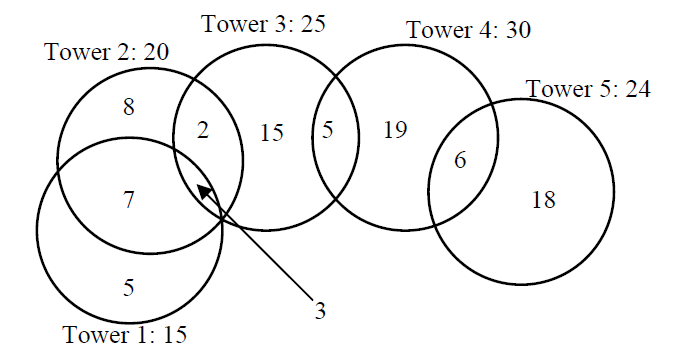
\includegraphics[width=0.6 \textwidth]{2005j.png}
					\caption{} \label{2005j}
				\end{figure}
				
				$M \le N \le 20,
					%, M \le 10
				 K \le 10$。
			\subsubsection{算法讨论}
				为了处理方便,先把有交集的部分从各个基站的人数中扣除。
				
				不妨直接枚举选择了哪 $M$ 个点,再枚举这 $K$ 个有交集的地方,看看其中是否有一个点(或更多)被选择。若是,则将交集的人数加回答案,取最优值返回。
				
				可将选择的点和每处交集涉及的基站用位
				% 运算
				表示出,加快速度。	
			\subsubsection{时空复杂度}
				时间复杂度 $\mathcal{O}\left(\binom{N}{M} \cdot N K \right)$。配合位运算,速度超快。
					
				空间复杂度 $\mathcal{O}\left(KN\right)$。
\newpage